%%%%%%%%%%%%%%%%%%%%%%%%%%%%%%%%%%%%%%%%%
% Beamer Presentation
% LaTeX Template
% Version 1.0 (10/11/12)
%
% This template has been downloaded from:
% http://www.LaTeXTemplates.com
%
% License:
% CC BY-NC-SA 3.0 (http://creativecommons.org/licenses/by-nc-sa/3.0/)
%
%%%%%%%%%%%%%%%%%%%%%%%%%%%%%%%%%%%%%%%%%

%----------------------------------------------------------------------------------------
%	PACKAGES AND THEMES
%----------------------------------------------------------------------------------------

\documentclass[UTF8,aspectratio=169,14pt]{ctexbeamer}

\usepackage{hyperref}
\hypersetup{
	colorlinks=true,
	linkcolor=red,
	anchorcolor=blue,
	citecolor=green
}

\mode<presentation> {
	
	% The Beamer class comes with a number of default slide themes
	% which change the colors and layouts of slides. Below this is a list
	% of all the themes, uncomment each in turn to see what they look like.
	
	%\usetheme{default}
	%\usetheme{AnnArbor}
	%\usetheme{Antibes}
	%\usetheme{Bergen}
	%\usetheme{Berkeley}
	%\usetheme{Berlin}
	%\usetheme{Boadilla}
	%\usetheme{CambridgeUS}
	%\usetheme{Copenhagen}
	%\usetheme{Darmstadt}
	%\usetheme{Dresden}
	%\usetheme{Frankfurt}
	%\usetheme{Goettingen}
	%\usetheme{Hannover}
	%\usetheme{Ilmenau}
	%\usetheme{JuanLesPins}
	%\usetheme{Luebeck}
	\usetheme{Madrid}
	%\usetheme{Malmoe}
	%\usetheme{Marburg}
	%\usetheme{Montpellier}
	%\usetheme{PaloAlto}
	%\usetheme{Pittsburgh}
	%\usetheme{Rochester}
	%\usetheme{Singapore}
	%\usetheme{Szeged}
	%\usetheme{Warsaw}
	
	% As well as themes, the Beamer class has a number of color themes
	% for any slide theme. Uncomment each of these in turn to see how it
	% changes the colors of your current slide theme.
	
	%\usecolortheme{albatross}
	%\usecolortheme{beaver}
	%\usecolortheme{beetle}
	%\usecolortheme{crane}
	%\usecolortheme{dolphin}
	%\usecolortheme{dove}
	%\usecolortheme{fly}
	%\usecolortheme{lily}
	%\usecolortheme{orchid}
	%\usecolortheme{rose}
	%\usecolortheme{seagull}
	%\usecolortheme{seahorse}
	%\usecolortheme{whale}
	%\usecolortheme{wolverine}
	
	%\setbeamertemplate{footline} % To remove the footer line in all slides uncomment this line
	%\setbeamertemplate{footline}[page number] % To replace the footer line in all slides with a simple slide count uncomment this line
	
	%\setbeamertemplate{navigation symbols}{} % To remove the navigation symbols from the bottom of all slides uncomment this line
}

\usepackage{graphicx} % Allows including images
\graphicspath{{./figs/}}
\usepackage{booktabs} % Allows the use of \toprule, \midrule and \bottomrule in tables
\usepackage{longtable}
\usepackage{listings}
\usepackage{xcolor}
\lstset{numbers=left, %设置行号位置
	numberstyle=\tiny, %设置行号大小
	keywordstyle=\color{blue}, %设置关键字颜色
	commentstyle=\color[cmyk]{1,0,1,0}, %设置注释颜色
	frame=single, %设置边框格式
	escapeinside=``, %逃逸字符(1左面的键),用于显示中文
	%breaklines, %自动折行
	extendedchars=false, %解决代码跨页时,章节标题,页眉等汉字不显示的问题
	xleftmargin=2em,xrightmargin=2em, aboveskip=1em, %设置边距
	tabsize=4, %设置tab空格数
	showspaces=false %不显示空格
}
% Fonts
% \usepackage{libertine}
% \setmonofont{Courier}
\setCJKsansfont[ItalicFont=Noto Serif CJK SC Black, BoldFont=Noto Sans CJK SC Black]{Noto Sans CJK SC}


%----------------------------------------------------------------------------------------
%	TITLE PAGE
%----------------------------------------------------------------------------------------

\title[第3讲]{第3讲 中断、异常和系统调用} % The short title appears at the bottom of every slide, the full title is only on the title page
\subtitle{第三节:中断处理机制--Detail}
\author{向勇、陈渝} % Your name
\institute[清华大学] % Your institution as it will appear on the bottom of every slide, may be shorthand to save space
{
清华大学计算机系 \\ % Your institution for the title page
\medskip
\textit{xyong,yuchen@tsinghua.edu.cn} % Your email address
}
\date{\today} % Date, can be changed to a custom date

\begin{document}

\begin{frame}
\titlepage % Print the title page as the first slide
\end{frame}

%----------------------------------------------------------------------------------------
%\begin{frame}
%\frametitle{提纲} % Table of contents slide, comment this block out to remove it
%\tableofcontents % Throughout your presentation, if you choose to use \section{} and \subsection{} commands, these will automatically be printed on this slide as an overview of your presentation
%\end{frame}

%----------------------------------------------------------------------------------------
%	PRESENTATION SLIDES
%----------------------------------------------------------------------------------------


%------------------------------------------------
\begin{frame}[plain,t]
	\frametitle{中断处理机制--建立中断服务例程}
	%	\framesubtitle{xxxx}
	\begin{columns}
		
		\begin{column}{0.4\textwidth}
			\centering
			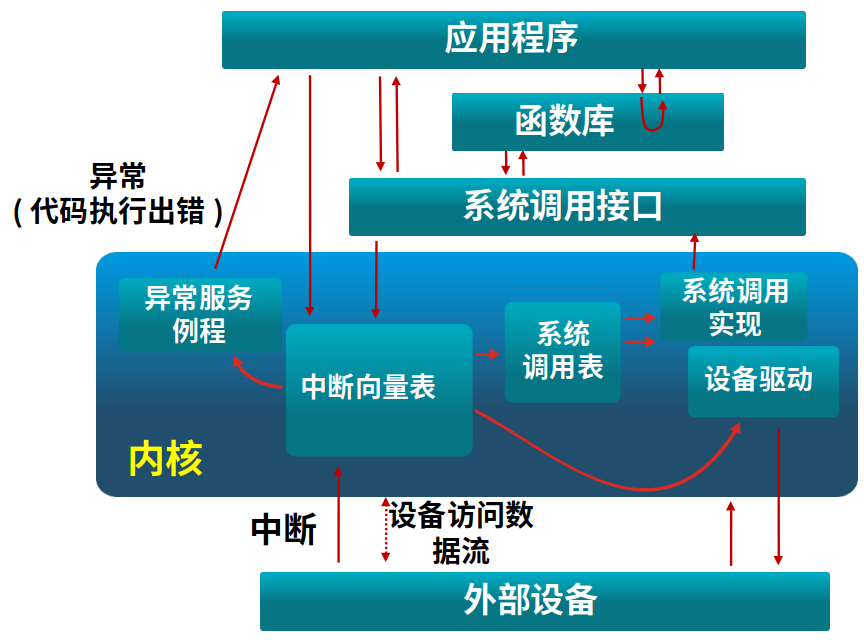
\includegraphics[width=1.0\linewidth]{os-4-intr-syscall-except}
			\begin{itemize} \small
				\item Core Local	Interruptor (CLINT)
				\item Platform-Level Interrupt Controller (PLIC)
			\end{itemize}
			
		\end{column}
		
		\begin{column}{0.6\textwidth}
			
			\centering
			%			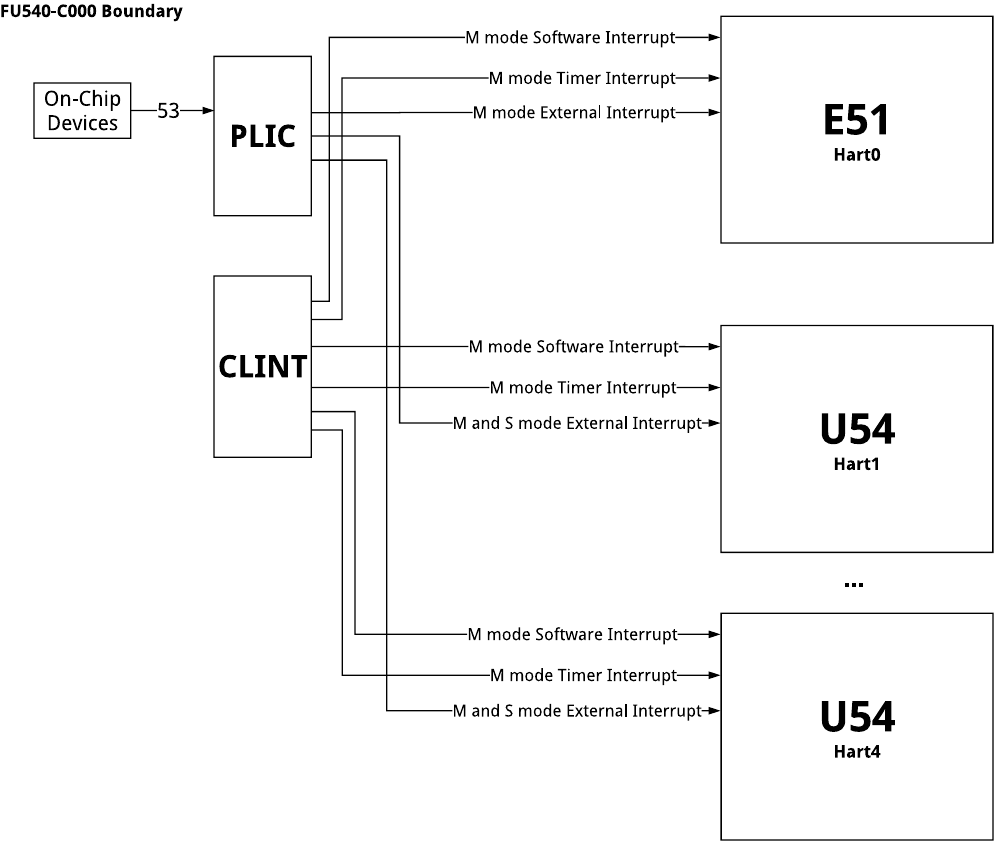
\includegraphics[width=.6\linewidth]{fu540-intr-arch}	
			
			
\includegraphics[width=1.\linewidth]{showmethecode}
			%show rcore tutorial	
		
		\end{column}
		
	\end{columns}
	
\end{frame}


%------------------------------------------------
\begin{frame}[plain,t]
	\frametitle{中断处理机制--建立中断服务例程}
	%	\framesubtitle{xxxx}
	\begin{columns}
		
		\begin{column}{0.45\textwidth}
			\centering
			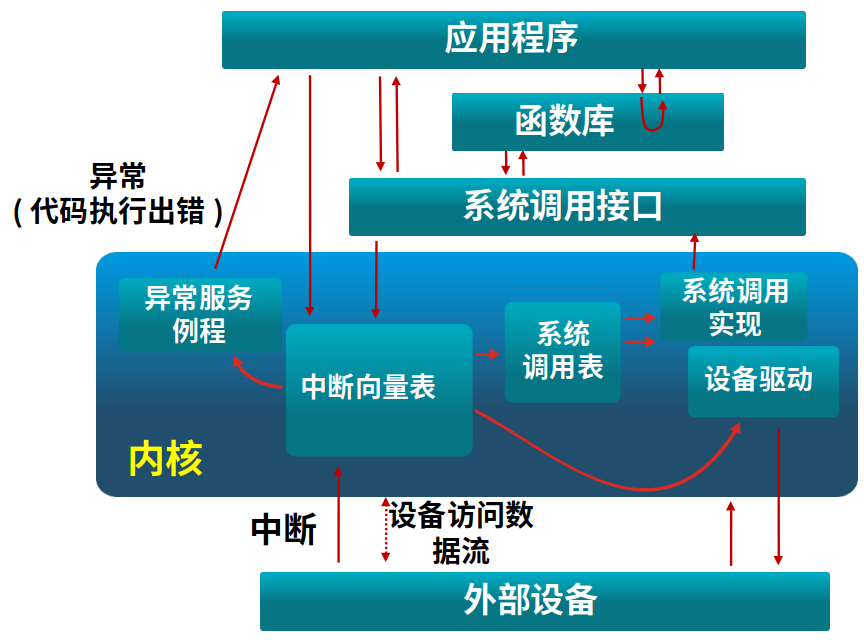
\includegraphics[width=1.0\linewidth]{os-4-intr-syscall-except}
			\begin{itemize} \small
				\item Core Local	Interruptor (CLINT)
				\item Platform-Level Interrupt Controller (PLIC)
			\end{itemize}
			
		\end{column}
		
		\begin{column}{0.5\textwidth}
			
			%			\centering
			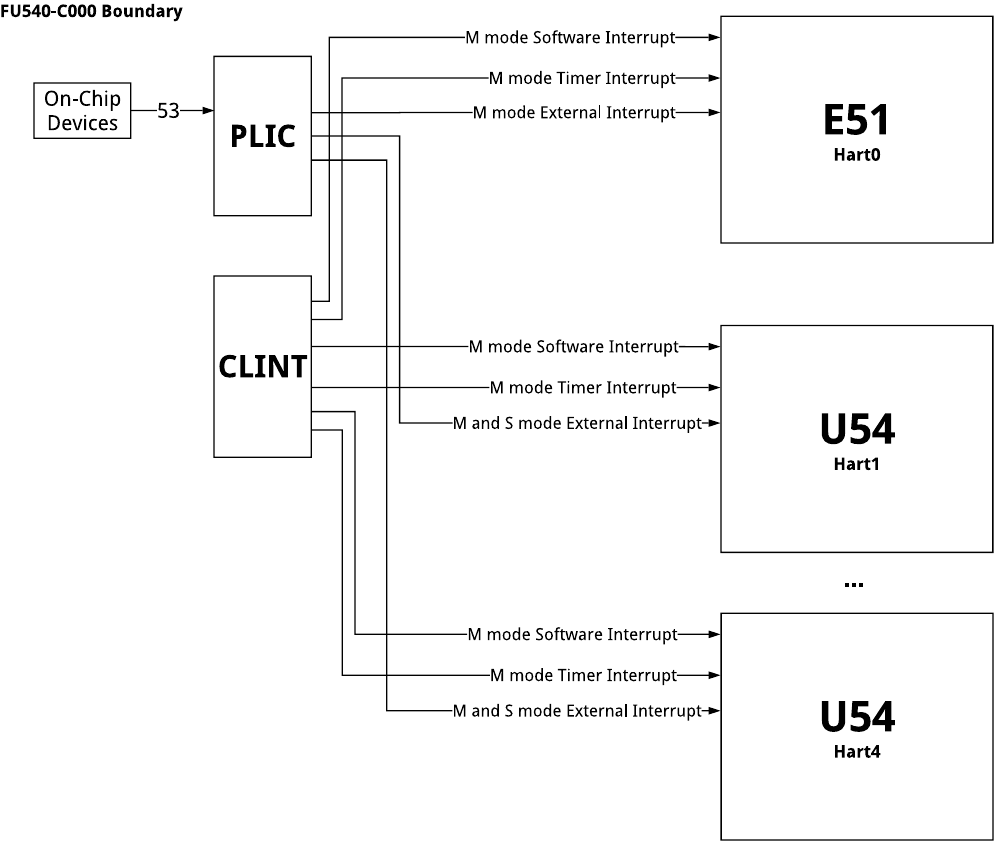
\includegraphics[width=1.\linewidth]{fu540-intr-arch}	
%			\centering
%			\LARGE 建立中断机制 \pause
%			
%			\Large
%			\begin{itemize}
%				\item 建立中断服务例程	 \pause
%				\item 让CPU能响应中断 \pause
%				\item 响应并处理中断 \pause
%				\item 保存/恢复现场 
%			\end{itemize}		
			
		\end{column}
		
	\end{columns}
	
\end{frame}



%------------------------------------------------
\begin{frame}[plain,t]
	\frametitle{中断处理机制--建立中断服务例程}
	%	\framesubtitle{xxxx}
	\begin{columns}
		
		\begin{column}{0.45\textwidth}
			\centering
			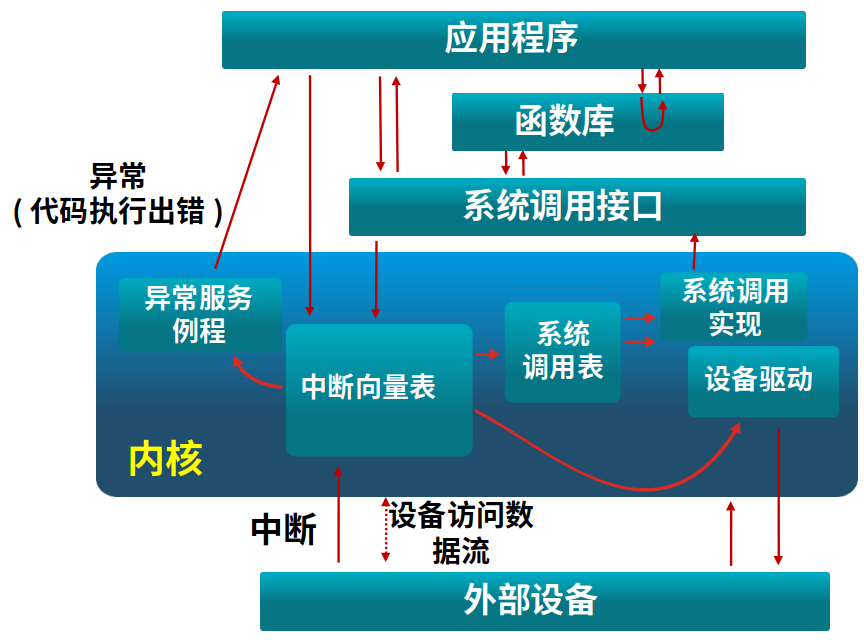
\includegraphics[width=1.0\linewidth]{os-4-intr-syscall-except}
			\begin{itemize} \small
				\item Core Local	Interruptor (CLINT)
				\item Platform-Level Interrupt Controller (PLIC)
			\end{itemize}
			
		\end{column}
		
		\begin{column}{0.5\textwidth}
			
			\centering
			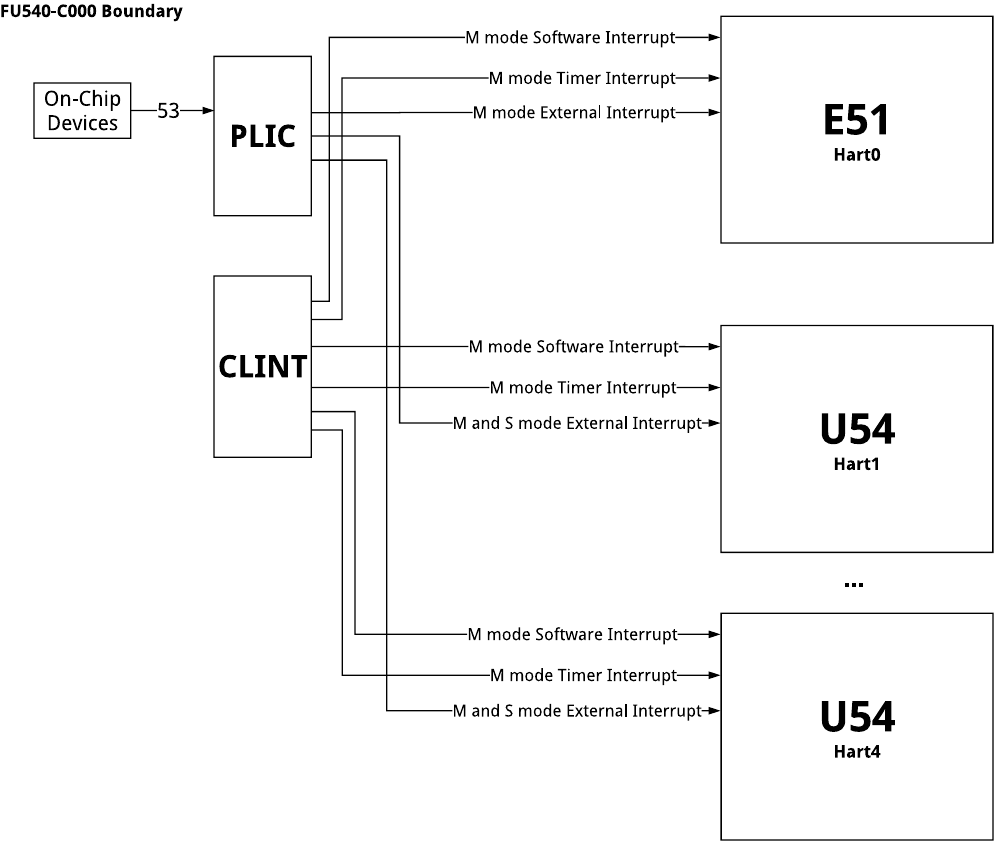
\includegraphics[width=.6\linewidth]{fu540-intr-arch}	
			
			
\includegraphics[width=.3\linewidth]{timer}
			%show rcore tutorial	
			
		\end{column}
		
	\end{columns}
	
\end{frame}


%------------------------------------------------
\begin{frame}[plain,t]
	\frametitle{中断处理机制--建立中断服务例程}
	%	\framesubtitle{xxxx}
	\begin{columns}
		
		\begin{column}{0.45\textwidth}
			\centering
			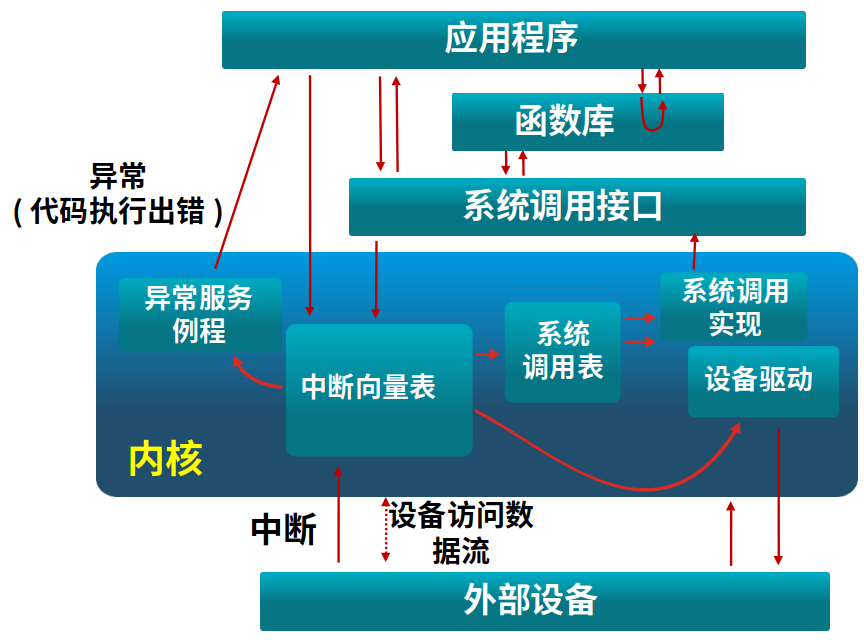
\includegraphics[width=1.0\linewidth]{os-4-intr-syscall-except}
			\begin{itemize} \small
				\item Core Local	Interruptor (CLINT)
				\item Platform-Level Interrupt Controller (PLIC)
			\end{itemize}
			
		\end{column}
		
		\begin{column}{0.5\textwidth}
			
			\centering
%			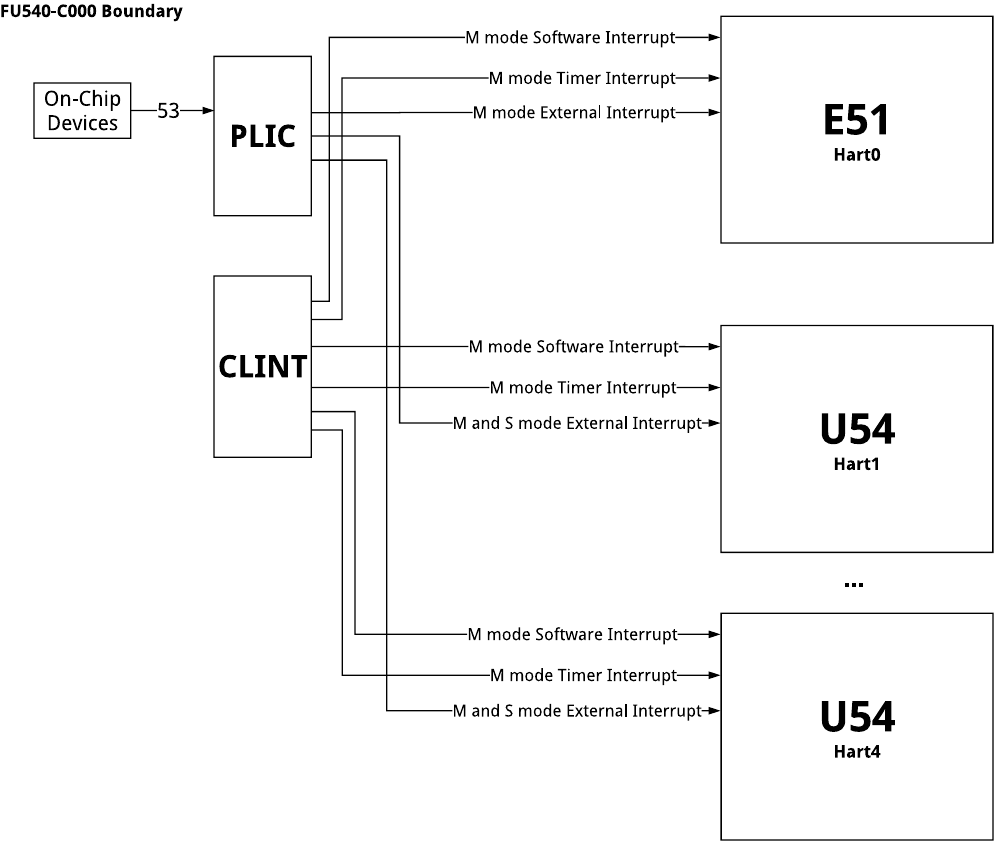
\includegraphics[width=.6\linewidth]{fu540-intr-arch}	
			
			
\includegraphics[width=.3\linewidth]{timer}
			%show rcore tutorial	
			
			\begin{itemize} \small 
				\item 初始化:设置时钟中断触发次数  \pause
				\item 初始化:设置 sie 的 TI 使能 STIE 位  \pause
				\item 服务例程:调用 OpenSBI 提供的接口设置下次时钟中断触发时间
			\end{itemize}
		    
		\end{column}
		
	\end{columns}
	
\end{frame}



%----------------------------------------------------------------------------------------

\end{document}
